\chapter{Pruebas Experimentales}

\section{Mecanismos de medición para la fase de pruebas}
Para este trabajo se realizaron dos tipos de prueba: pruebas de experiencia de usuario mediante las cuales, se busca obtener retroalimentación por parte de potenciales usuarios, de manera que el desarrollador pueda identificar errores y/o posibles cambios que pudieran hacerse al producto. \\

Como mecanismo de medición para las pruebas de experiencia de usuario, se emplea el método de validación de la metodología de Design Sprint de Google ® Ventures\cite{web16}. El proceso de validación se compone de dos partes:\\
\begin{enumerate}
    \item Pruebas de usuario.
    \item Retroalimentación de los stakeholders.
\end{enumerate}
Después de la finalización del prototipo se procede a realizar pruebas. Una simple prueba de usuario permite descubrir información valiosa rápidamente. Ayuda a responder preguntas como ¿Qué es lo que los usuarios disfrutan o no gustan del prototipo? ¿Qué les gustaría que mejorara? \\

Después se continúa con la validación de los interesados o accionistas (stakeholders). Estas personas son el director de la Escuela Superior de Medicina, profesores del área de morfología y los alumnos de la misma. \\

Para motivos de este trabajo y los tiempos que se viven, el stakeholder será el mismo estudiante que presenta este trabajo, ya que resulta imposible hacer pruebas con los usuarios potenciales debido a la situación de epidemia nacional por el virus SARS-COV-2.\\

De igual forma se tomará en cuenta la retroalimentación de los sinodales y directores del proyecto mismo. Así, la revisión y aprobación de estos es esencial para que la validación se considere exitosa.\\

\section{Pruebas de Entorno 3D con headset de R.V.}
A continuación, se mostrarán las pruebas no automatizadas realizadas a las características, cada prueba está relacionada a un feature o features específicos, los cuales fueron probados conforme fueron desarrollados bajo el flujo de trabajo Git Flow\cite{pathania2017elements}.\\ 

Se detalla que es lo que se espera conseguir y bajo qué condiciones se consigue este objetivo, así como se indica si la característica ha pasado la prueba o la ha fallado. Así mismo se incluyen capturas de pantallas que muestran el funcionamiento de la característica y observaciones particulares a la prueba, indicando según lo requiera detalles de implementación o configuración.\\

\subsection{Configuración de entradas}
\begin{itemize}
    \item \textbf{id de Develop Realizados}
    \begin{itemize}
        \item 1
    \end{itemize}
    \item \textbf{Descripción de la Prueba}
    \begin{itemize}
        \item Configurar la entrada de movimiento de los controles Oculus Touch ®. 
    \end{itemize}
    \item \textbf{Condiciones de la Prueba}
    \begin{itemize}
        \item El usuario, desde una posición inicial, realiza el movimiento del control izquierdo y derecho, uno a la vez, en el espacio en tres dimensiones moviéndose en los tres ejes X, Y y Z. Recibiendo el movimiento de los mismos y este será mostrado dentro del HMD, demostrado por el placeholder de ambos controles.\\
    \end{itemize}
    \item \textbf{Observaciones}
    \begin{itemize}
        \item A pesar de que aún no se utilizan todos los entradas que ofrece el control Oculus Touch ® el rastreo de los controles en el espacio funciona correctamente, esto nos sirve para desarrollar a futuro las siguientes características adicionales.\\
        A continuación se muestra la ejemplificación de el movimiento que se realiza y el cual es mostrado posteriormente dentro del sistema.        
    \end{itemize}
    \item \textbf{Estado}
    \begin{itemize}
        \item Aprobado
    \end{itemize}
    \item \textbf{Capturas de Pantalla}
    \begin{figure}[H]
       	\begin{center}
       		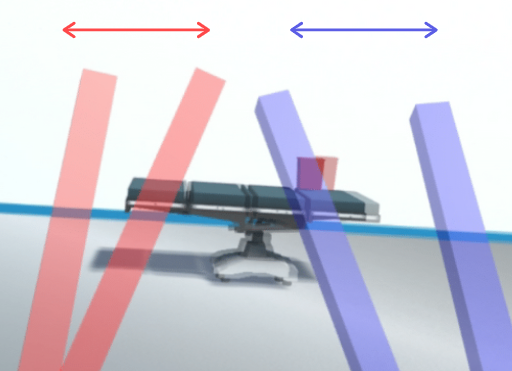
\includegraphics[width = .7\textwidth]{source/images/image60.png}
       		\captionof{figure}{\label{fig:im41}Placeholders con forma de prismas rectangulares representando y mostrando el movimiento de las manos con los controles Oculus Touch.}
       	\end{center} 
    \end{figure}
\end{itemize}

\subsection{Teleportación}
\begin{itemize}
    \item \textbf{id de Develop Realizados}
    \begin{itemize}
        \item 2
    \end{itemize}
    \item \textbf{Descripción de la Prueba}
    \begin{itemize}
        \item Prueba de en la cual el sistema es capaz de emitir una curva indicadora que emana desde el  placeholder del usuario hacia un destino requerido por el mismo. 
    \end{itemize}
    \item \textbf{Condiciones de la Prueba}
    \begin{itemize}
        \item El usuario, desde una posición inicial, toca el stick de cualquier control y realiza el movimiento del control izquierdo o derecho, uno a la vez, dirigiendo el arco  de indicación de localización de teleportación en el espacio en tres dimensiones moviéndose en los tres ejes X, Y y Z, moviendo este hacia el lugar deseado dentro del entorno 3D  y al dejar de tocarlo este deberá de desaparecer inmediatamente. Este será mostrado por el HMD, demostrado la capacidad de realizar la llamada de estos elementos.\\
    \end{itemize}
    \item \textbf{Observaciones}
    \begin{itemize}
        \item Al tocar el stick de cualquiera de los controles se emite una curva para determinar una próxima función de teleportación, el arco creado es claro y útil para determinar la localización y este se mueve dependiendo de la distancia y ángulo en el cual sea invocado. Puede que sea poco necesario que el usuario pueda utilizar ambos controles para la misma función.
    \end{itemize}
    \item \textbf{Estado}
    \begin{itemize}
        \item Aprobado
    \end{itemize}
    \item \textbf{Capturas de Pantalla}
    \begin{figure}[H]
       	\begin{center}
       		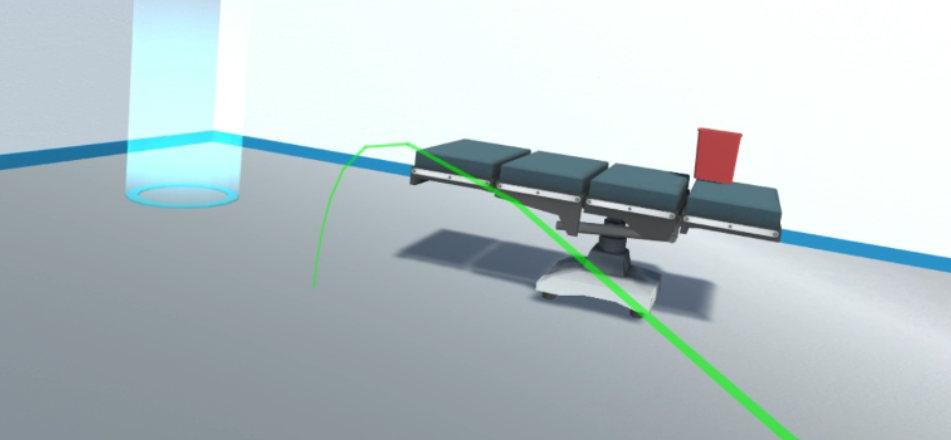
\includegraphics[width = .7\textwidth]{source/images/image27.png}
       		\captionof{figure}{\label{fig:im42}Línea verde indicadora desde el placeholder hacía un punto en el entorno virtual(Simulando una trayectoria)}
       	\end{center} 
    \end{figure}
\end{itemize}

\begin{itemize}
    \item \textbf{id de Develop Realizados}
    \begin{itemize}
        \item 3
    \end{itemize}
    \item \textbf{Descripción de la Prueba}
    \begin{itemize}
        \item Prueba de la capacidad de que el sistema permite el movimiento dentro del entorno virtual mediante teleportación.
    \end{itemize}
    \item \textbf{Condiciones de la Prueba}
    \begin{itemize}
        \item 
        El usuario, desde una posición inicial, toca el stick de cualquier control y realiza el movimiento del control izquierdo o derecho, uno a la vez, dirigiendo el arco de indicación de localización de teleportación en el espacio en tres dimensiones moviéndose en los tres ejes X, Y y Z, indicando la localización hacia la cual desea y presionando el stick respectivo para realizar la acción de teleportación. Recibiendo el movimiento de los mismos y este será mostrado dentro del HMD, demostrado por la nueva ubicación en el entorno virtual.\\        
    \end{itemize}
    \item \textbf{Observaciones}
    \begin{itemize}
        \item Ya se utilizan más entradas del control Oculus Touch ® estas pueden llegar a no ser tan intuitivas y presentar dificultades de ejecución para el usuario. La curva indicando la dirección y la posterior reubicación de del usuario en la ubicación previamente elegida por el mismo.
    \end{itemize}
    \item \textbf{Estado}
    \begin{itemize}
        \item Aprobado
    \end{itemize}
    \item \textbf{Capturas de Pantalla}
    \begin{figure}[H]
       	\begin{center}
       		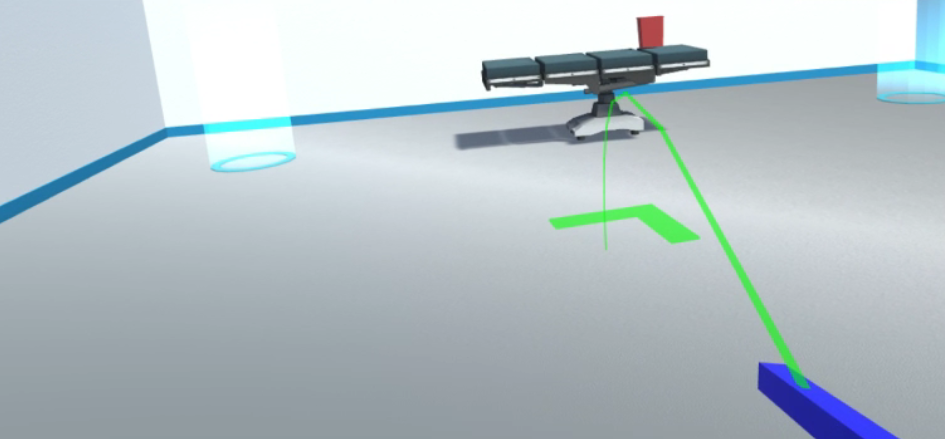
\includegraphics[width = .7\textwidth]{source/images/image12.png}
       		\captionof{figure}{\label{fig:im43}Uso de la curva indicadora para especificar un lugar y una orientación hacia donde se teleportará el usuario.}
       	\end{center} 
    \end{figure}
\end{itemize}

\begin{itemize}
    \item \textbf{id de Develop Realizados}
    \begin{itemize}
        \item 3
    \end{itemize}
    \item \textbf{Descripción de la Prueba}
    \begin{itemize}
        \item Prueba de la capacidad de que el sistema permite el movimiento dentro del entorno virtual mediante teleportación.
    \end{itemize}
    \item \textbf{Condiciones de la Prueba}
    \begin{itemize}
        \item 
        El usuario, desde una posición inicial, toca el stick de cualquier control y realiza el movimiento del control izquierdo o derecho, uno a la vez, dirigiendo el arco de indicación de localización de teleportación en el espacio en tres dimensiones moviéndose en los tres ejes X, Y y Z, indicando la localización hacia la cual desea y presionando el stick respectivo para realizar la acción de teleportación. Recibiendo el movimiento de los mismos y este será mostrado dentro del HMD, demostrado por la nueva ubicación en el entorno virtual.\\        
    \end{itemize}
    \item \textbf{Observaciones}
    \begin{itemize}
        \item Ya se utilizan más entradas del control Oculus Touch ® estas pueden llegar a no ser tan intuitivas y presentar dificultades de ejecución para el usuario. La curva indicando la dirección y la posterior reubicación de del usuario en la ubicación previamente elegida por el mismo.
    \end{itemize}
    \item \textbf{Estado}
    \begin{itemize}
        \item Aprobado
    \end{itemize}
    \item \textbf{Capturas de Pantalla}
    \begin{figure}[H]
       	\begin{center}
       		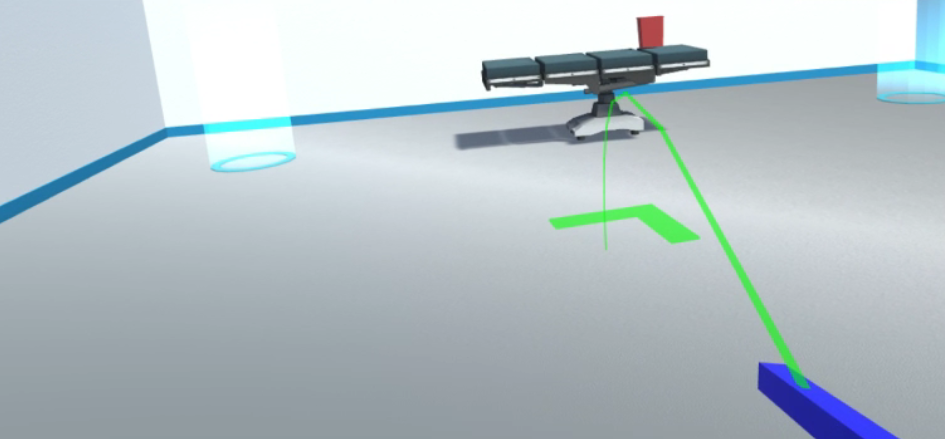
\includegraphics[width = .7\textwidth]{source/images/image12.png}
       		\captionof{figure}{\label{fig:im44}Uso de la curva indicadora para especificar un lugar y una orientación hacia donde se teleportará el usuario.}
       	\end{center} 
    \end{figure}
\end{itemize}

\begin{itemize}
    \item \textbf{id de Develop Realizados}
    \begin{itemize}
        \item 4
    \end{itemize}
    \item \textbf{Descripción de la Prueba}
    \begin{itemize}
        \item El usuario puede elegir la dirección en la cual desea reaparecer después invocar la teleportación, esto será indicado mediante una flecha la cual hará referencia a la dirección  la cual el usuario habrá determinado anteriormente.
    \end{itemize}
    \item \textbf{Condiciones de la Prueba}
    \begin{itemize}
        \item El usuario, desde una posición inicial, toca el stick de cualquier control y realiza el movimiento del control izquierdo o derecho, uno a la vez, dirigiendo el arco de indicación de localización de teleportación en el espacio en tres dimensiones moviéndose en los tres ejes X, Y y Z, indicando la localización hacia la cual desea, posteriormente moviendo el stick en los ejes X y Z para elegir la dirección en la cual quiere mirar al determinar el proceso de teleportación,  posteriormente soltando el stick respectivo para realizar la acción de teleportación. Recibiendo el movimiento de los mismos y este será mostrado dentro del HMD, demostrado por la nueva ubicación y dirección en el entorno virtual.        
    \end{itemize}
    \item \textbf{Observaciones}
    \begin{itemize}
        \item Se ha actualizado la manera de interactuar con el proceso de teleportación, así este se pretende que sea más intuitivo para el usuario reduciendo la capacidad de movimientos posibles y agregando controles que ayudan a la inmersión en el entorno virtual.
    \end{itemize}
    \item \textbf{Estado}
    \begin{itemize}
        \item Aprobado
    \end{itemize}
    \item \textbf{Capturas de Pantalla}
    \begin{figure}[H]
       	\begin{center}
       		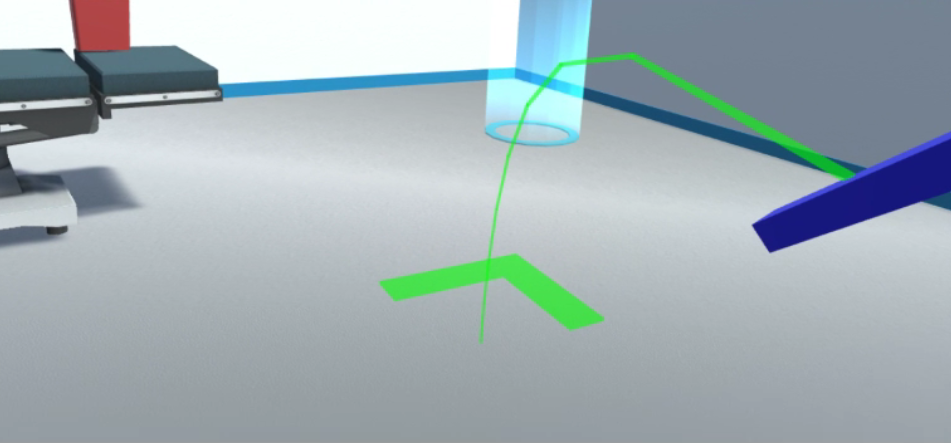
\includegraphics[width = .7\textwidth]{source/images/image46.png}
       		\captionof{figure}{\label{fig:im45} Flecha verde en el punto de teleportación, indicadora de la dirección hacia donde estará orientado el usuario una vez teletransportado.}
       	\end{center} 
    \end{figure}
\end{itemize}

\begin{itemize}
    \item \textbf{id de Develop Realizados}
    \begin{itemize}
        \item 5
    \end{itemize}
    \item \textbf{Descripción de la Prueba}
    \begin{itemize}
        \item Funcionamiento correcto de puntos de teleportación.
    \end{itemize}
    \item \textbf{Condiciones de la Prueba}
    \begin{itemize}
        \item 
        El usuario, desde una posición inicial, toca el stick de cualquier control y realiza el movimiento del control izquierdo o derecho, uno a la vez, dirigiendo el arco de indicación de localización de teleportación en el espacio en tres dimensiones moviéndose en los tres ejes X, Y y Z, indicando la localización hacia la cual punto de teleportación desea, posteriormente moviendo el stick en los ejes X y Z para elegir la dirección en la cual quiere mirar al determinar el proceso de teleportación, posteriormente presionando el stick respectivo para realizar la acción de teleportación. Recibiendo el movimiento de los mismos y este será mostrado dentro del HMD, demostrado por la nueva ubicación y dirección en el entorno virtual.       
    \end{itemize}
    \item \textbf{Observaciones}
    \begin{itemize}
        \item Se ha actualizado la manera de interactuar con el proceso de teleportación, así este se pretende que sea más intuitivo para el usuario reduciendo la capacidad de movimientos posibles y agregando controles que ayudan a la inmersión en el entorno virtual.La utilidad de los puntos de teleportación y su uso depende del diseño que haya disponible en el entorno virtual, estos pueden resultar muy beneficioso en el momento de resaltar un lugar el cual se quiere que el usuario se acerque para que realice una situación específica en el sitio de interés.
    \end{itemize}
    \item \textbf{Estado}
    \begin{itemize}
        \item Aprobado
    \end{itemize}
    \item \textbf{Capturas de Pantalla}
    \begin{figure}[H]
       	\begin{center}
       		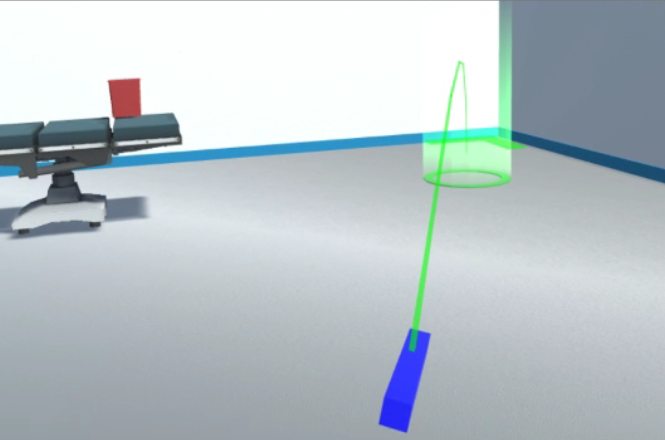
\includegraphics[width = .7\textwidth]{source/images/image68.png}
       		\captionof{figure}{\label{fig:im46} Punto de teleportación marcando un lugar lugar en específico y preestablecido hacia donde se teleportará.}
       	\end{center} 
    \end{figure}
\end{itemize}

\begin{itemize}
    \item \textbf{id de Develop Realizados}
    \begin{itemize}
        \item 6
    \end{itemize}
    \item \textbf{Descripción de la Prueba}
    \begin{itemize}
        \item El usuario puede cambiar de dirección de orientación sin la necesidad de realizar una teleportación.
    \end{itemize}
    \item \textbf{Condiciones de la Prueba}
    \begin{itemize}
        \item El usuario, desde una posición inicial, mueve el stick del control izquierdo en los ejes X y Z recibiendo el movimiento del mismos y este será mostrado dentro del HMD generando una pequeña alteración de orientación en los ejes antes mencionados.
    \end{itemize}
    \item \textbf{Observaciones}
    \begin{itemize}
        \item 
    \end{itemize}
    \item \textbf{Estado}
    \begin{itemize}
        \item Aprobado
    \end{itemize}
    \item \textbf{Capturas de Pantalla}
    \begin{figure}[H]
       	\begin{center}
       		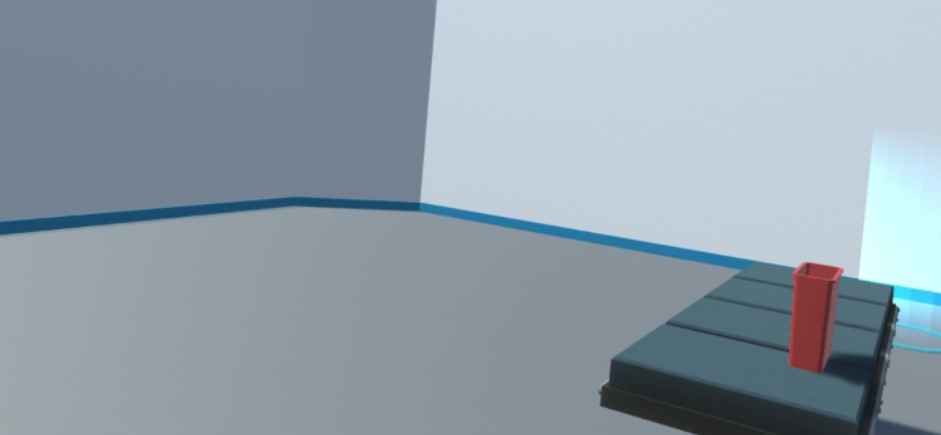
\includegraphics[width = .7\textwidth]{source/images/image66.png}
       		\captionof{figure}{\label{fig:im47}Vista descriptiva hacia una orientación en específico. }
       	\end{center} 
    \end{figure}

    \begin{figure}[H]
        \begin{center}
            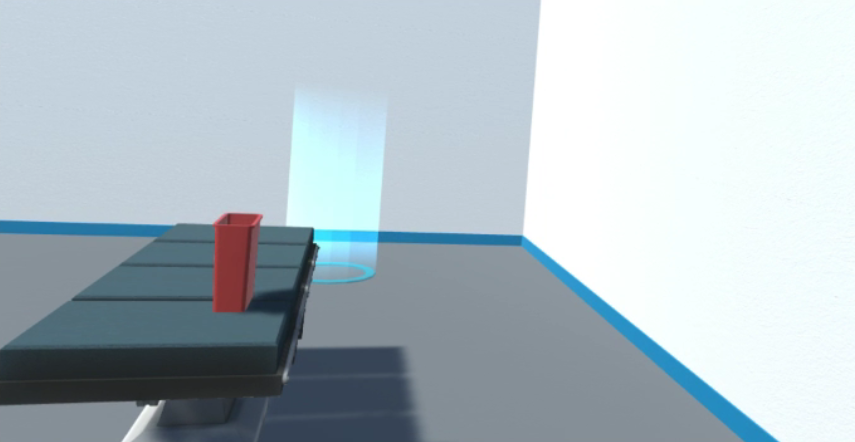
\includegraphics[width = .7\textwidth]{source/images/image38.png}
            \captionof{figure}{\label{fig:im48} Vista descriptiva de un cambio de orientación respecto a la imagen anterior. Sin necesidad de teleportarse.}
        \end{center} 
 \end{figure}
\end{itemize}

\begin{itemize}
    \item \textbf{id de Develop Realizados}
    \begin{itemize}
        \item 7
    \end{itemize}
    \item \textbf{Descripción de la Prueba}
    \begin{itemize}
        \item El usuario no es capaz de introducirse en el entorno virtual en lugares no admitidos por el programa, así como permite.
    \end{itemize}
    \item \textbf{Condiciones de la Prueba}
    \begin{itemize}
        \item El usuario, después de haberse desplazado de una posición inicial, con los comandos anteriormente mencionados intenta explorar fuera del entorno virtual “exponiendo” su cabeza fuera de los límites del entorno designado, lo cual causará una oclusión del entorno para evitar que este pueda salir del área designada.
        Asimismo con objetos en los cuales queremos que pueda ver a través de ellos quedan exentos de las limitaciones anteriores.     
    \end{itemize}
    \item \textbf{Observaciones}
    \begin{itemize}
        \item 
    \end{itemize}
    \item \textbf{Estado}
    \begin{itemize}
        \item Aprobado
    \end{itemize}
    \item \textbf{Capturas de Pantalla}
    \begin{figure}[H]
       	\begin{center}
       		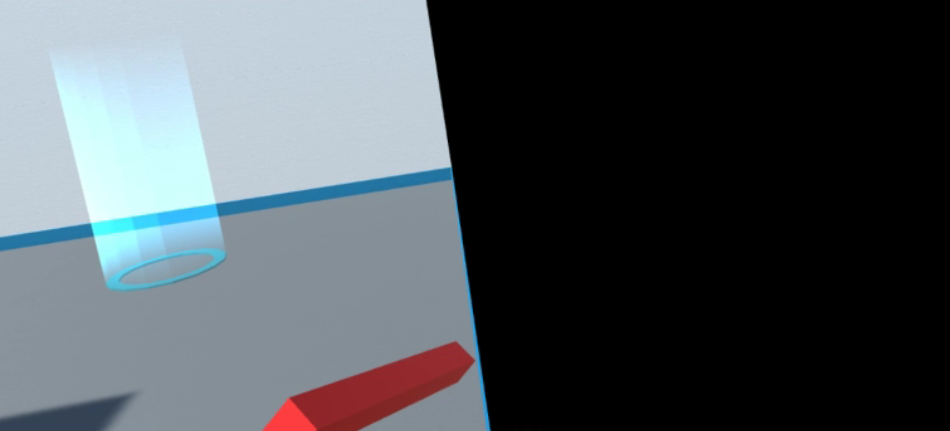
\includegraphics[width = .7\textwidth]{source/images/image39.png}
       		\captionof{figure}{\label{fig:im49}Vista descriptiva del impedimento hacia afuera del entorno virtual admitido.}
       	\end{center} 
    \end{figure}
    \begin{figure}[H]
        \begin{center}
            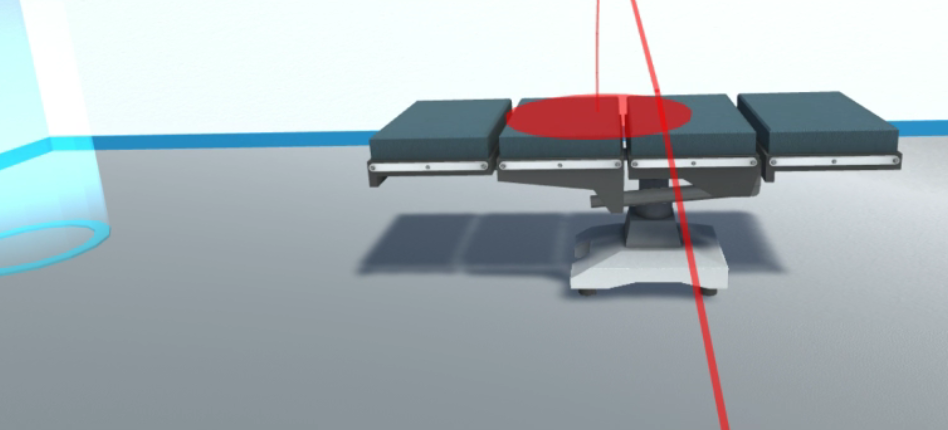
\includegraphics[width = .7\textwidth]{source/images/image28.png}
            \captionof{figure}{\label{fig:im410}Punto rojo sobre una superficie no permitida en el entorno virtual, impidiendo la teleportación.}
        \end{center} 
    \end{figure}
    \begin{figure}[H]
        \begin{center}
            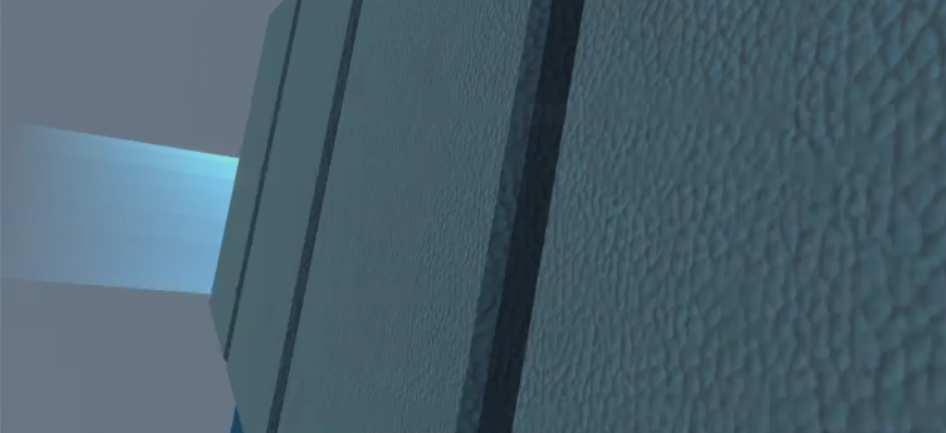
\includegraphics[width = .7\textwidth]{source/images/image34.png}
            \captionof{figure}{\label{fig:im411}Vista del usuario antes de intentar introducirse a un entorno virtual no permitido.}
        \end{center} 
    \end{figure}
    \begin{figure}[H]
        \begin{center}
            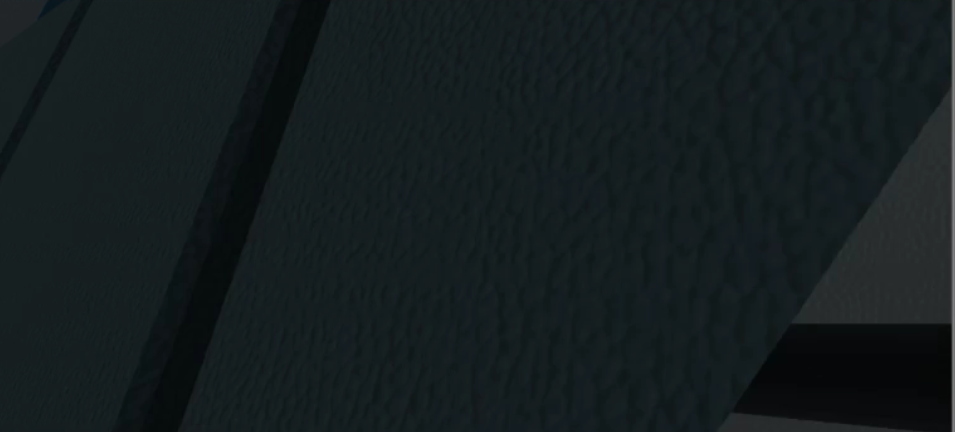
\includegraphics[width = .7\textwidth]{source/images/image8.png}
            \captionof{figure}{\label{fig:im412}Vista del usuario intentando introducirse a un entorno virtual no permitido. La vista se empieza a oscurecer.}
        \end{center} 
    \end{figure}
    \begin{figure}[H]
        \begin{center}
            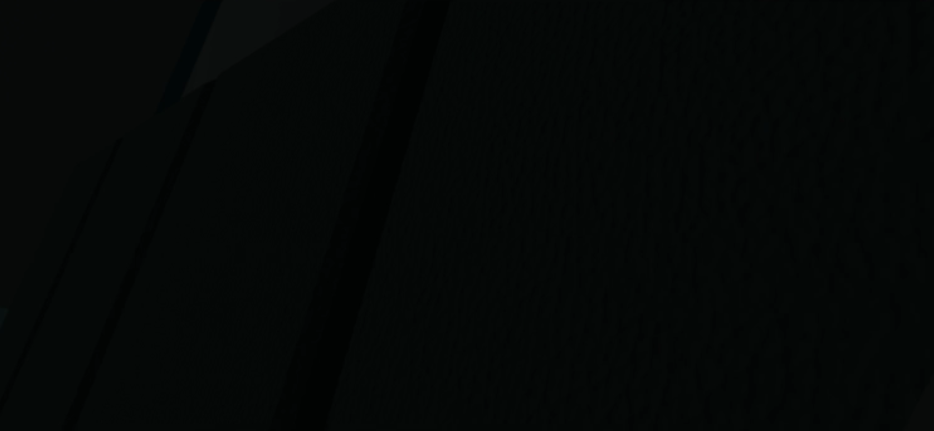
\includegraphics[width = .7\textwidth]{source/images/image58.png}
            \captionof{figure}{\label{fig:im413}Vista del usuario introduciéndose en un entorno virtual no permitido, la vista está completamente oscura}
        \end{center} 
    \end{figure}

    
    
\end{itemize}

\section{Presencia e interacción de manos}
\begin{itemize}
    \item \textbf{id de Develop Realizados}
    \begin{itemize}
        \item 8
    \end{itemize}
    \item \textbf{Descripción de la Prueba}
    \begin{itemize}
        \item El usuario es capaz de realizar los movimientos permitidos de las manos haciendo uso de los botones y sensores de los controles. 
    \end{itemize}
    \item \textbf{Condiciones de la Prueba}
    \begin{itemize}
        \item Los modelos virtuales de las manos imitan los movimientos que son realizados al tomar los controles e interactuar con los sensores y botones de los mismos, estos son limitados pero las acciones asemeja el movimiento de la mano de manera consistente e interactiva. Acciones como señalar, tomar, saludar, levantar dedos están incluidas dentro de este y son apreciadas por el usuario en el HMD en cuanto estas acciones son realizadas.
    \end{itemize}
    \item \textbf{Observaciones}
    \begin{itemize}
        \item Los movimientos se encuentran limitados a las capacidades del control mismo, aunque comparados con interacciones ”antiguas” de realidad virtual, estas proveen una experiencia de inmersión más real dentro del sistema de realidad virtual.
    \end{itemize}
    \item \textbf{Estado}
    \begin{itemize}
        \item Aprobado
    \end{itemize}
    \item \textbf{Capturas de Pantalla}
    \begin{figure}[H]
       	\begin{center}
       		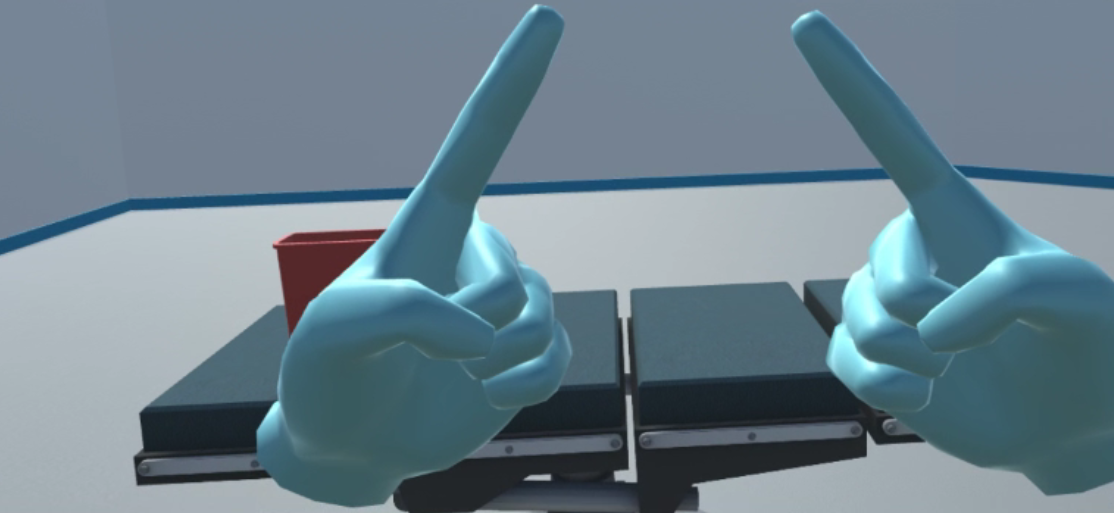
\includegraphics[width = .7\textwidth]{source/images/image32.png}
       		\captionof{figure}{\label{fig:im414}Modelo de manos, mostrando cómo se alza el dedo índice cuando el usuario lo hace a través de los sensores y botones del control.}
       	\end{center} 
    \end{figure}
    \begin{figure}[H]
        \begin{center}
            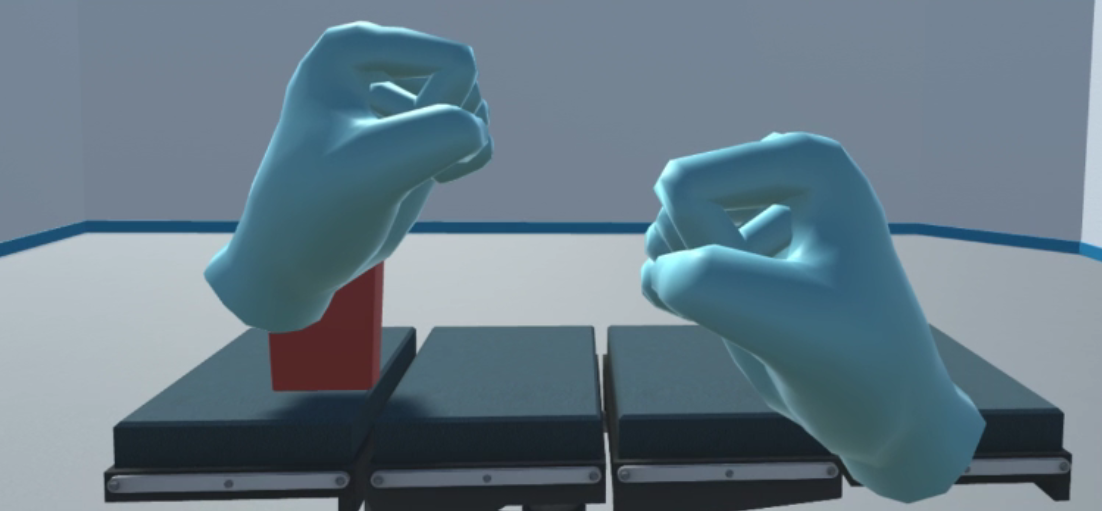
\includegraphics[width = .7\textwidth]{source/images/image7.png}
            \captionof{figure}{\label{fig:im415}Modelo de manos, mostrando la mano cerrada cuando el usuario lo hace a través de los sensores y botones del control.}
        \end{center} 
 \end{figure}
\end{itemize}

\subsection{Interactuando con entorno}
\begin{itemize}
    \item \textbf{id de Develop Realizados}
    \begin{itemize}
        \item 9
    \end{itemize}
    \item \textbf{Descripción de la Prueba}
    \begin{itemize}
        \item El usuario es capaz de tomar objetivos específicos designados como pruebas de entorno con las manos.
    \end{itemize}
    \item \textbf{Condiciones de la Prueba}
    \begin{itemize}
        \item Al acercarse a un objeto de prueba específico el usuario es capaz de tomarlos e inspeccionarlos.  Al tomarlo debe de ser capaz de dejar el objeto en un lugar diferente del cual fue tomado.
    \end{itemize}
    \item \textbf{Observaciones}
    \begin{itemize}
        \item Las características de un objeto, entiéndase, que este pueda ser interactuado con las manos virtuales pueden ser transferidas a más modelos 3D lo cual nos da la libertad de interacción con una mayor cantidad de objetos.
        La prueba fue realizada exitosamente.      
    \end{itemize}
    \item \textbf{Estado}
    \begin{itemize}
        \item Aprobado
    \end{itemize}
    \item \textbf{Capturas de Pantalla}
    \begin{figure}[H]
       	\begin{center}
       		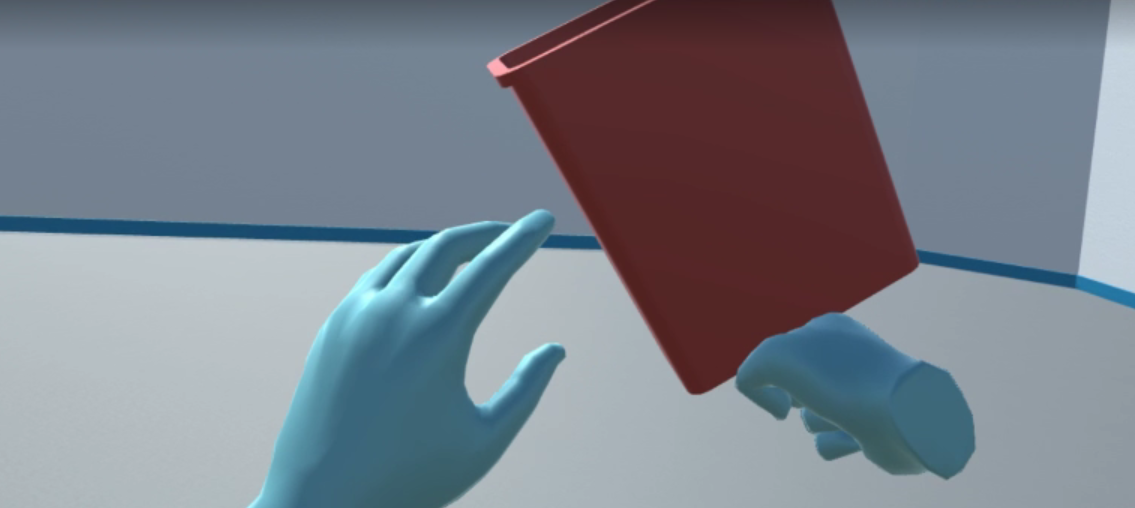
\includegraphics[width = .7\textwidth]{source/images/image11.png}
       		\captionof{figure}{\label{fig:im416}Previo a la toma de un objeto}
       	\end{center} 
    \end{figure}
    \begin{figure}[H]
        \begin{center}
            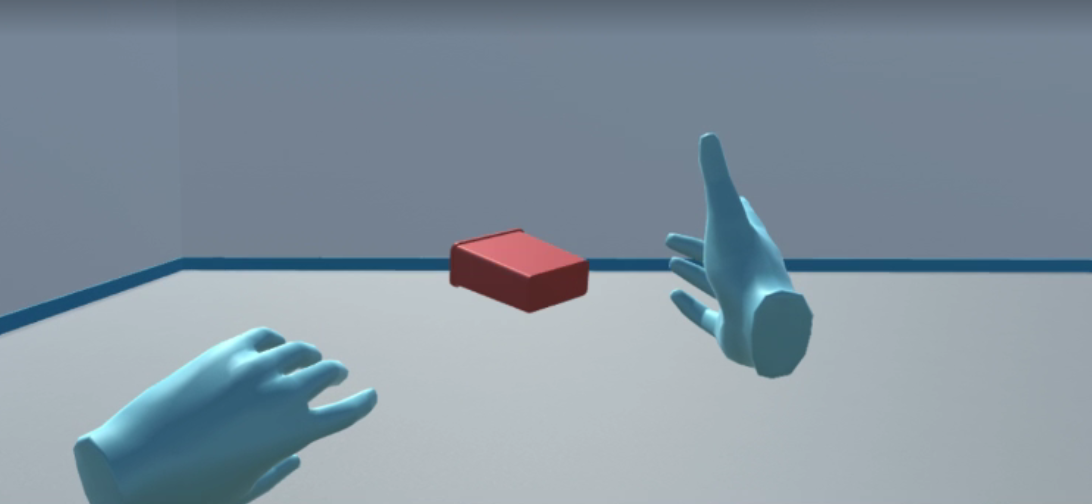
\includegraphics[width = .7\textwidth]{source/images/image43.png}
            \captionof{figure}{\label{fig:im417}Toma de un objeto antes y después de lanzarlo}
        \end{center} 
    \end{figure}
\end{itemize}

\subsection{Interacciones manuales adicionales}
\begin{itemize}
    \item \textbf{id de Develop Realizados}
    \begin{itemize}
        \item 10
    \end{itemize}
    \item \textbf{Descripción de la Prueba}
    \begin{itemize}
        \item El usuario es capaz de cambiar de manos el objeto que se tiene tomado y de arrojar el mismo para proveer una experiencia más interactiva dentro del entorno virtual.
    \end{itemize}
    \item \textbf{Condiciones de la Prueba}
    \begin{itemize}
        \item El usuario debe de tomar un objeto interactivo con una mano y después de esto cambiará de mano el objeto, posteriormente dejará el objeto y lo tomará de nuevo con la mano y lo arrojará frente a él.
    \end{itemize}
    \item \textbf{Observaciones}
    \begin{itemize}
        \item Las características de un objeto, entiéndase, que este pueda ser interactuado con las manos virtuales pueden ser transferidas a más modelos 3D lo cual nos da la libertad de interacción con una mayor cantidad de objetos.      
    \end{itemize}
    \item \textbf{Estado}
    \begin{itemize}
        \item Aprobado
    \end{itemize}
    \item \textbf{Capturas de Pantalla}
    \begin{figure}[H]
       	\begin{center}
       		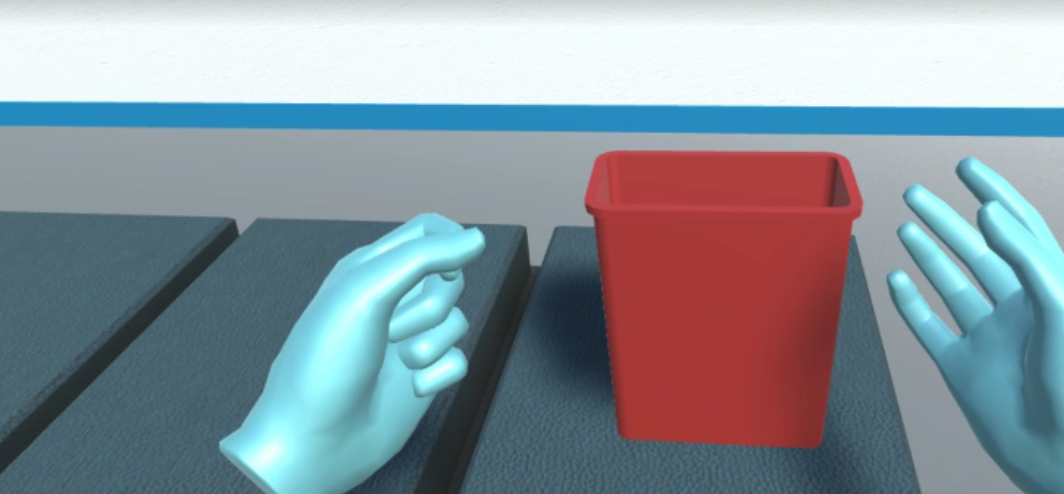
\includegraphics[width = .7\textwidth]{source/images/image76.png}
       		\captionof{figure}{\label{fig:im418}Muestra las manos y un objeto antes de ser tomado por las manos}
       	\end{center} 
    \end{figure}
    \begin{figure}[H]
        \begin{center}
            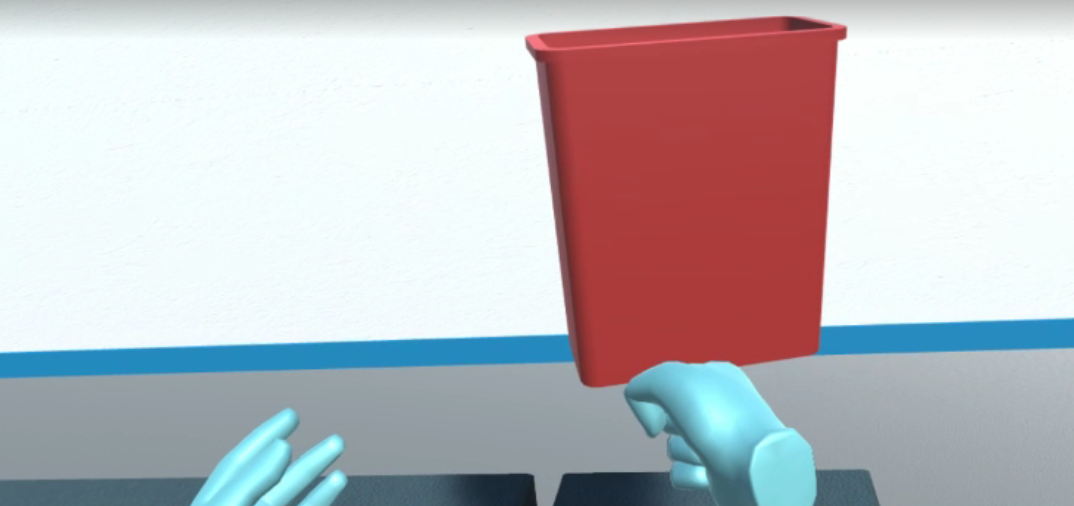
\includegraphics[width = .7\textwidth]{source/images/image6.png}
            \captionof{figure}{\label{fig:im419}Una mano tomando y levantando el objeto}
        \end{center} 
    \end{figure}
    \begin{figure}[H]
        \begin{center}
            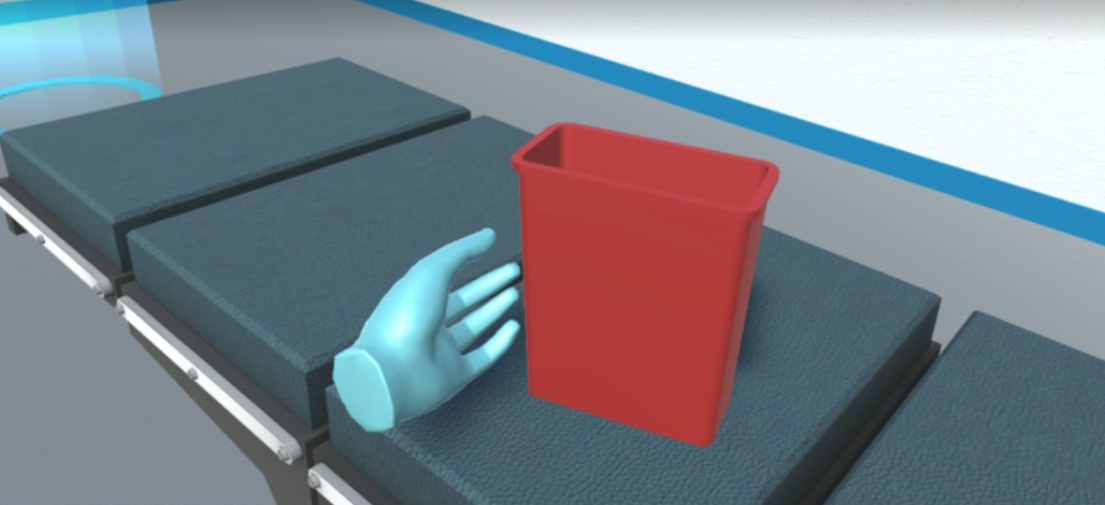
\includegraphics[width = .7\textwidth]{source/images/image64.png}
            \captionof{figure}{\label{fig:im420}Después de pasar el objeto de una mano a otra se vuelve a soltar en un lugar distinto en el que estaba.}
        \end{center} 
    \end{figure}
\end{itemize}

\section{Retroalimentación de los stakeholders y usuarios potenciales}
Debido a la situación global que se ha vivido durante el año 2020 comenzando en el mes de marzo la posibilidad de realizar pruebas presenciales con los stakeholders y usuarios potenciales se vio mermada de gran manera, lo cual desembocó en poca retroalimentación por parte de los usuarios finales, profesor de seguimiento, directores y sinodales. \\

Los problemas que surgieron son inherentes a la naturaleza del proyecto mismo, ya que al ser un sistema de realidad virtual, para ser probado se necesita la presencia física del usuario para que éste evalúe y experimente el sistema con todas sus características, así como sus capacidades y áreas de oportunidad en las cuales se debería de invertir más tiempo o cambios que se requieran realizar para mejorar el resultado final del proyecto, esto dependiendo completamente de la experiencia  de uso que el stakeholder obtenga al realizar las pruebas con el sistema mismo.\\

Por lo tanto toda la retroalimentación del proyecto proviene únicamente del desarrollador, afectando el resultado final y dejando una versión menos refinada del mismo.\\
